\section{Design grafico}
\subsection{Palette di colori}
I colori tentano di richiamare quelli tipici degli animali domestici, con tonalità calde e accoglienti.
\begin{adjustwidth}{1cm}{1cm}
    \centering
    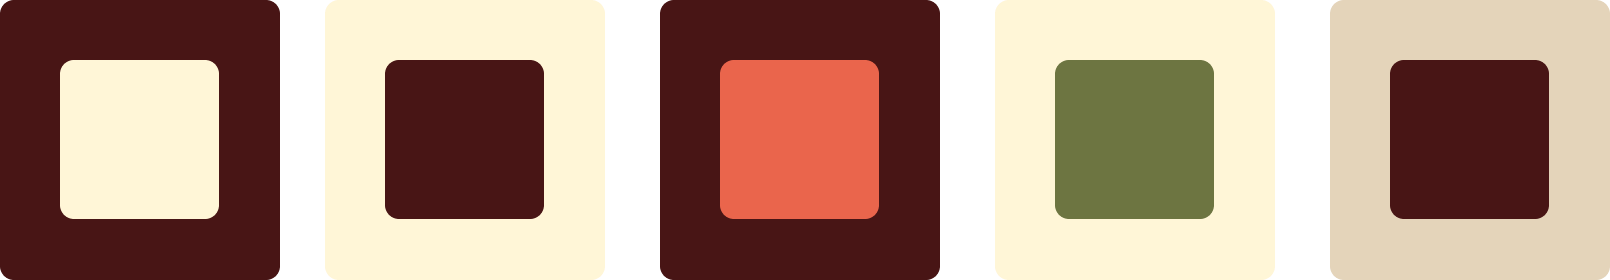
\includegraphics[width=0.8\textwidth]{assets/palette.png}
\end{adjustwidth}
 La palette principale, in modalità giorno (\textit{light mode}), include:
\begin{itemize}
    \item \textbf{Colore primario: \cbox{beige} \#FFF6D7 (Beige)} - un colore chiaro e neutro che offre un buon contrasto con gli altri colori
    \item \textbf{Colore secondario 1: \cbox{brown} \#481515 (Marrone)} - un marrone scuro utilizzato per elementi di testo o background secondari.
    \item \textbf{Colore di accento: \cbox{orange} \#EA654C (Arancione)} - principalmente per elementi interattivi come pulsanti e link.
    \item \textbf{Colore secondario 2: \cbox{grey} \#E4D4BA (Grigio)} - un colore neutro che fornisce contrasto e aiuta a creare separazione visiva tra gli elementi.
    \item \textbf{Colore secondario 3: \cbox{green} \#6D7541 (Verde)} - un colore neutro che richiama la natura. Utilizzato principalmente per elementi decorativi.
\end{itemize}
\paragraph{Per l'accessibilità}:
le seguenti informazioni sono state verificate utilizzando diversi strumenti, in ultimo il tool \textit{Color Contrast} di Silktide.
\begin{center}
\setcounter{table}{1} 
\begin{tabular}{|p{4.5cm}|p{4.5cm}|p{2cm}|p{2.5cm}|}
\hline
\rowcolor{brown}
\color{white}\textbf{Colore 1} & 
\color{white}\textbf{Colore 2} & 
\color{white}\textbf{Contrasto} & 
\color{white}\textbf{Accessibilità} \\
\hline
\rowcolor{beige} \cbox{beige} Beige (\#FFF6D7) & \cbox{brown} Marrone (\#481515) & 13.93:1 & Raggiunto AA e AAA \\
\hline
\rowcolor{beige} \cbox{beige} Beige (\#FFF6D7) & \cbox{orange} Arancione (\#EA654C) & 3.00:1 & Zona grigia (*) \\
\hline
\rowcolor{beige} \cbox{beige} Beige (\#FFF6D7) & \cbox{green} Verde (\#6D7541) & 4.55:1 & Raggiunto AA \\
\hline
\rowcolor{beige} \cbox{brown} Marrone (\#481515) & \cbox{orange} Arancione (\#EA654C) & 4.65:1 & Raggiunto AA \\
\hline
\rowcolor{beige} \cbox{brown} Marrone (\#481515) & \cbox{green} Verde (\#6D7541) & 3.06:1 & Zona grigia (*) \\
\hline
\rowcolor{beige} \cbox{grey} Grigio (\#E4D4BA) & \cbox{brown} Marrone (\#481515) & 10.35:1& Raggiunto AA e AAA\\
\hline
\end{tabular}
\captionof{table}{Verifiche di contrasto colori. NOTA: Non sono riportate le combinazioni di colori che non sono state usate come testo e background insieme o tra link visitato e non visitato.}
\end{center}
\begin{adjustwidth}{1cm}{1cm}
    \textmd{(*) A causa di limiti troppo stringenti delle WCAG, trovare un contrasto sufficiente con tutti i colori risulta quasi impossibile. Il contrasto baige e arancione è stato usato per link visitati e non visitati su sfondo scuro, altrimenti viene usato marrone e verde su sfondo chiaro. Abbiamo sottolineato i link per sopperire ad eventuali problemi di contrasto.}
\end{adjustwidth}
Poichè ci siamo concentrate sull'accessibilità della palette nella modalità light mode, la dark mode (che rispecchia una scelta dell'utente, per quanto possibile) è stata progettata cercando di mantenere un buon contrasto tra gli elementi, tuttavia non è assicurato che tutte le combinazioni di colori rispettino gli standard di accessibilità.
\subsection{Font}
Il carattere tipografico selezionato per questo progetto è Parkinsans, un font sans geometrico e moderno, reperibile gratuitamente sulla piattaforma Google Fonts al seguente link \href{https://fonts.google.com/specimen/Parkinsans}{fonts.google.com/Parkinsans}.
Il font utilizzato vuole essere chiaro e leggibile, pur mantenendo un aspetto giocoso e amichevole. \\
\textbf{Il nome stesso del font rivela la sua nobile origine:} è stato infatti progettato dall'agenzia londinese Red Stone per l'associazione britannica \textit{Parkinson’s UK}, con l'obiettivo di rispondere alle sfide visive e cognitive poste dalla malattia, tenendo conto di sintomi come lentezza di elaborazione, difficoltà di attenzione e alterazioni visuo-percettive, che possono rendere la lettura un'attività faticosa anche in assenza di un vero deficit visivo o disurbo specifico (come la dislessia). \\\\
Per le pagine di stampa abbiamo optato per un comune font serif, Times New Roman, per facilitare la lettura su carta stampata.
\begin{adjustwidth}{1cm}{1cm}
    \centering
    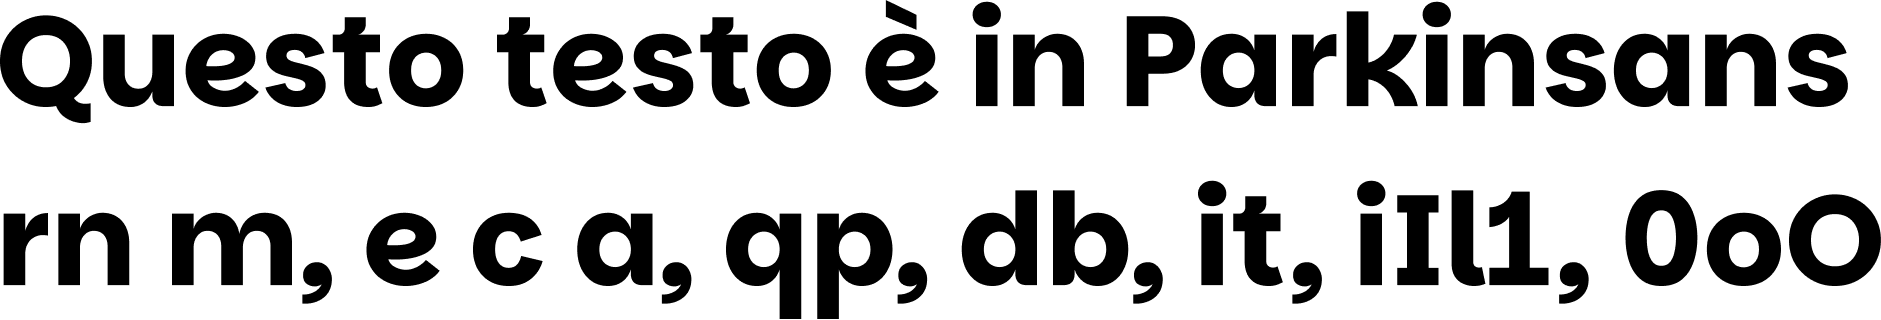
\includegraphics[width=0.8\textwidth]{assets/esempio_parkinsans.png}
\end{adjustwidth}
\paragraph{Verifiche di accessibilità}
\begin{itemize}
    \item controllo apertura delle lettere (e, c, a);
    \item controllo legature tra caratteri (qp, db, rn);
    \item controllo differenza tra lettere simili (iIl1, oO0);
    \item controllo spaziatura tra parole.
\end{itemize}
\subsection{Scelte stilistiche nella divisione utente / amministratore}
Il layout e in generale il design grafico delle pagine dedicate agli amministratori si presenta più sobrio e formale rispetto a quello delle pagine utente, per sottolineare la differenza di ruolo e responsabilità tra i due tipi di utenti.\\
Un esempio di differenza di layout, oltre alla nav, è l'assenza del footer nelle pagine amministratore, che risulterebbe superfluo, distraente e ingombrante.\\
\begin{mdframed}[
    backgroundcolor=gray!15,
    linecolor=none,
    leftmargin=-3cm,
    rightmargin=-3cm,
    innerleftmargin=4cm,
    innerrightmargin=4cm,
    innertopmargin=10pt,
    innerbottommargin=10pt
]
\textmd{In generale nella sezione admin abbiamo rilassato alcune best practice di accessibilità, questo perchè l'area amministratore non è destinata ad un pubblico generico.}\\
Per esempio nella sezione riservata, le attività da completare hanno il testo in piccolo, si presume che col tempo l'amministratore non abbia più necessità di leggere continuamente a quale attività corrisponde ogni link.\\
Altre differenze sono state descritte nella sezione \ref{sec:accessibilita}{ Accessibilità}.
\end{mdframed}
\subsection{Logo}
Il logo, utilizzato in più varianti, raffigura un cuore realizzato con le sagome di due tipici segnaposto di mappe. Una strada collega il cuore ad una casa stilizzata posta alla destra in lontananza. \\
L'idea è quella di rappresentare il significato del sito web con un singolo simbolo: il cuore rappresenta l'amore e l'affetto che gli utenti cercano per i loro animali, mentre i segnaposto simboleggiano la localizzazione geografica che, grazie alla piattaforma, può essere superata, arrivando idealmente fino alla casa dell'utente.\\
\begin{center}
    
\includegraphics[width=5cm]{assets/dark-mode-logo.png}
\end{center}
Un significato alternativo ma dualmente significativo è quello per cui gli animali portano amore nelle case degli utenti, rappresentato dalla strada che collega il cuore alla casa.\\
\begin{mdframed}[
    backgroundcolor=gray!15,
    linecolor=none,
    leftmargin=-3cm,
    rightmargin=-3cm,
    innerleftmargin=4cm,
    innerrightmargin=4cm,
    innertopmargin=10pt,
    innerbottommargin=10pt
]
\textmd{Il logo di PetMatch è stato realizzato senza l'ausilio di strumenti di intelligenza artificiale, utilizzando esclusivamente inventiva personale e software di grafica vettoriale.}
\end{mdframed}
\subsection{Le immagini}
\textbf{Le illustrazioni} tentano di essere inclusive rappresentando persone di diverse etnie, generi di età e anche persone con mobilità ridotta. Le immagini in questione si trovano alle pagine di registrazione e login, lavora con noi, e nel form di adozione degli animali.\\
Le \textbf{fotografie degli animali} presenti sul sito web sono immagini reali dei nostri personali amici animali o di quelli di compagni umani a noi vicini.\\
\textbf{Altre immagini} sono state reperite da siti web che offrono immagini gratuite e libere da diritti d'autore come \url{https://it.freepik.com/}. \\
Infine è presente un'immagine generata dall'intelligenza artificiale, specificamente nella sezione "Come funziona". Nell'immagine è raffigurato un furgone tipico del trasporto animale, con la scritta PetMatch e colori coerenti con la palette del sito web. Abbiamo deciso di inserire un'immagine (e non un'illustrazione) perchè rappresenta un elemento di contesto alla credibilità del servizio. Per trasparenza è visibile un piccolo watermark nell'angolo in basso a destra dell'immagine, che indica il contenuto generato da AI.\\
\begin{mdframed}[
    backgroundcolor=gray!15,
    linecolor=none,
    leftmargin=-3cm,
    rightmargin=-3cm,
    innerleftmargin=4cm,
    innerrightmargin=4cm,
    innertopmargin=10pt,
    innerbottommargin=10pt
]
\textmd{Le illustrazioni sono state create senza l'ausilio di strumenti di intelligenza artificiale, utilizzando esclusivamente inventiva personale e software di grafica.}
\end{mdframed}
\subsection{Altre scelte di design grafico}
Oltre alle illustrazioni, alcune scelte di design particolari:
\begin{itemize}
    \item navbar utente a forma di osso.
    \item il tasto torna sù, a sagoma di gatto che si anima al passaggio del mouse.
    \item footer che raffigurato come un terreno erboso.
\end{itemize}
\textbf{Home}
\begin{itemize}
    \item elementi grafici semplici e puliti per evitare distrazioni e facilitare la navigazione. In particolare, l'uso dell'icona della zampa segue un percorso di passi per invogliare l'utente allo scroll della pagina.
    \item una sezione che spiega il procedimento di adozione in 5 semplici passi, raffigurati come timeline e con gif animate visibili al passaggio del mouse.
    \item una sezione che mostra i prossimi eventi organizzati da PetMatch, in formati cartoline appese con delle mollette, ma soprattutto interattive: al passaggio del mouse, la cartolina svolazza simulando il vento.
    \item una sezione con i nostri sostenitori, raggruppati da un collare stilizzato (non costituisce un richiamo simbolico, ma è un elemento decorativo che richiama il mondo degli animali domestici).
\end{itemize}
Le altre pagine utente richiamano lo stile grafico della homepage, mantenendo coerenza visiva e facilità di navigazione.